\documentclass{article}

% Language setting
% Replace `english' with e.g. `spanish' to change the document language
\usepackage{polski}
\usepackage[utf8]{inputenc}
\usepackage[polish]{babel}
\usepackage{polski}


% Set page size and margins
% Replace `letterpaper' with `a4paper' for UK/EU standard size
\usepackage[letterpaper,top=2cm,bottom=2cm,left=3cm,right=3cm,marginparwidth=1.75cm]{geometry}

% Useful packages
\usepackage{amsmath}
\usepackage{graphicx}
\usepackage[colorlinks=true, allcolors=blue]{hyperref}
\usepackage{listings}
\usepackage{xcolor}
\usepackage{textcomp}
\usepackage{enumitem}
\usepackage{float}
\usepackage{hyperref}




\lstset{
  backgroundcolor=\color{white},
  basicstyle=\fontsize{0.02\textwidth}{0.02\textwidth}\selectfont\color{black}\ttfamily,
  keywordstyle=\color{cyan},
  commentstyle=\color{green},
  stringstyle=\color{magenta}
  literate={~}{$\sim$}{1} 
}

\begin{document}

\begin{titlepage}
	\begin{center}
     	\vspace*{1cm}
     	\huge\textbf{Sprawozdanie\\}
     	\vspace{0.3cm}
     	\huge{z Proejektu Indywidualnego:\\Konfiguracja mini serwera domowego na komputerze RPi4 - serwisy: SMB i Pi-hole\\}
       	\vspace{0.8cm}
       	\huge{Tomasz Kowalski 313565\\}
            \vspace{0.3cm}
            \huge{Informatyka Stosowana}
       	\vfill
       	\vspace{0.cm}
		
\includegraphics[scale=0.5]{EE.png} 
   	\end{center}
\end{titlepage}

\tableofcontents
\clearpage

\section{Wstęp, założenia}
Tematem projektu jest konfiguracja mini serwera domowego w oparciu o komputer jednopłytkowy Raspberry Pi 4. Założeniem jest stowrzyć dysk domowy NAS oraz utworzyć blokadę reklam dla sieci domowej.\\

Jest wiele gotowych dysków sieciowych np. Synology Nas, jednak jest to bardzo drogie rozwiązanie w porównaniu do RPi, zużywające więcej energi. Raspberry daje również dużo więcej innych możliwości, dlatego wybrałem ten komputer.\\

Do wykonania projektu wybrałem serwis SMB (Samba), ponieważ jest on bezpłatny i szeroko wspierane przez różne systemy operacyjne, w tym Windows, Mac OS i Linux. Serwis ten jest często uważany za łatwiejszy w konfiguracji niż niektóre inne protokoły, takie jak NFS czy FTP. Wspomniane protokoły również są darmowe i zawierają jeszcze funkcje, które nie będą używane. Dlatego do tej części projektu wybrałem serwis SMB.\\

Kolejnym wybranym oprogramowaniem jest Pi-hole, które blokuje reklamy, złośliwe czy śledźące oprogramowania w sieci blokując ich domeny. Pi-hole pełni funkcję serwera DNS i jest dedykowanym oprogramowaniem do Raspberry Pi. Inne dostępne oprogramowanie to AdGuard albo NextDNS, jednak nie są one dedykowane do systemów linuksowych i zajmują dużo miejsca. Zaletą Pi-hole jest prosta instalacja oraz konfiguracja i dostosowanie blokowania do własnych potrzeb.\\

Założeniem mojego projektu jest przygotowanie Raspberry do pracy w sieci domowej, zainstalowanie serwisu SMB oraz konfiguracja go do utworzenia dysku sieciowego NAS1 oraz instalacja i dostosowanie Pi-hole do moich potrzeb, utworzenie skryptów do realizacji powyższych zadań, aby łatwo i szybko odtworzyc pracę.\\
Sprawozdanie zawiera:
\begin{enumerate}[label=\textbullet]
  \item przygotowanie komputera do pracy
  \item opis zainstalowanyh oprogramowań
  \item dodanie dostępu poza siecią lokalną przy pomocy Tailscale
  \item skpryty konfiguracyjne
\end{enumerate}


\section{Dane techniczne sprzętu}
Parametry komputera:
\begin{lstlisting}
    urzadzenie:     Paspberry Pi 4 Model B
    architektura:   ARM v8
    procesor:       Broadcom BCM2711, quad-core Cortex-A72 64-bit SoC @ 1.5GHz
    pamiec RAM:     2GB LPDDR4
    zasilanie:      5V DC via USB-C connector (minimum 3A)
\end{lstlisting}
Parametry karty sieciowej:
\begin{lstlisting}
    rodzaj:         Wi-Fi 802.11b/g/n/ac (Wi-Fi 5)
    predkosc:       150 Mbps
    czestotliwosc:  2.4GHz i 5GHz (wykozystywana 2.4GHz)
    MAC:            dc:a6:32:2a:26:07
    IPv4:           192.168.0.3
\end{lstlisting}

\section{System operacyjny}
Na platformie Raspberry Pi istnieje szeroki wybór różnorodnych systemów operacyjnych do zainstalowania. Dostępne jest wiele wariantów opartych na Linuxie, takich jak Ubuntu, Arch Linux czy Rasbian, które cieszą się dużą popularnością. Dodatkowo, dostępny jest również Windows 10 IoT Core, specjalnie zoptymalizowany dla urządzeń Internetu Rzeczy, takich jak Raspberry Pi.\\

Zdecydowałem się na system Raspberry Pi OS (Rasbian), który jest oficjalne oprogramowanie opracowane przez Raspberry Pi Foundation. Jest on zaprojektowany specjalnie dla tej platformy, co gwarantuje optymalne działanie. Raspberry Pi OS jest rekomendowany dla większości zastosowań na Raspberry Pi.\\

Pierwszym krokiem przy instalacji było stworzenie nowego użytkownika oraz zainstalowanie wybranego systemu operacyjnego na karcie pamięci SD. Następnie, karta została umieszczona w module Raspberry Pi, a do urządzenia podłączony monitor oraz zasilanie. Po pierwszym uruchomieniu, system szybko się podnosi i pojawia się terminal.  Na samym początku warto przeprowadzić konfigurację podstawowych elementów urządzenia:

\begin{enumerate}[label=\textbullet]
  \item ustawienie statycznego adresu IP
  \item dodanie sieci domowej
  \item włączenie radia
  \item włączenie serwisu SSH
  \item ponowne uruchomienie
\end{enumerate}
Dzięki takiemu ustawieniu konfiguracji, samodzielnie nadajemy adres IP naszemu urządzeniu, zamiast nadawać go dynamicznie przez protokół DHCP. Gwarantuje to, że adres IP nie ulegnie zmianie. Warto wybrać numer IP spoza zakresu przydzielanego przez DHCP, żeby uniknąć konfliktów, ale jednocześnie upewnić się, że jest dostępny. Po przeprowadzeniu konfiguracji, możemy odłączyć monitor i korzystać z usługi SSH, umożliwiającą pracę zdalną z innego komputera w sieci.\\

Dołączony jest także skrypt konfiguracyjny o nazwie \textit{basic\_config.sh}, który wymaga wprowadzenia własnych wartości, takich jak statyczny adres IP, brama, serwery DNS, nazwa sieci czy hasło. Po ustanowieniu połączenia z internetem, ważne jest również zaktualizowanie systemu, żeby mieć najnowsze oprogramowanie.\cite{raspberrypi}


\section{Dysk sieciowy}
Aby utworzyć dysk sieciowy NAS1, wybrałem serwis SMB. Servis oferuje prostą konfigurację i szeroką kompatybilność z różnymi systemami operacyjnymi, w tym z systemami Windows, Mac i Linux. Może być łatwo skonfigurowany na domowym routerze lub serwerze NAS, umożliwiając udostępnianie plików i zasobów w sieci lokalnej. Serwis NFS, choć również popularny w środowiskach UNIX i Linux, może być mniej przystępny dla użytkowników domowych, zwłaszcza z systemami Windows. Wymaga dodatkowych narzędzi i konfiguracji, aby uzyskać pełną kompatybilność.\\

Kolejnym etapem jest instalacja oprogramowania. Po zakończeniu instalacji, konieczne jest przeprowadzenie kilku dodatkowych konfiguracji na urządzeniu Raspberry Pi:
\begin{enumerate}[label=\textbullet]
  \item utworzenie miejsca na mapowanie dysku zewnętrznego
  \item dodanie mapowania
  \item dodanie informacji o dysku do pliku konfiguracyjnego Samby
\end{enumerate}
Podczas konfiguracji, należy dostosować ustawienia dla konkretnego użytkownika. Jeśli chcemy stworzyć dysk domowy, można stworzyć nowego użytkownika o nazwie "domownicy", aby oddzielić jego część od reszty. Na końcu konieczne jest ustawienie hasła dla użytkownika do serwisu SMB.\\

Dzięki takiej konfiguracji, możliwe jest łatwe mapowanie dysku sieciowego w systemie operacyjnym Windows. Wystarczy podać adres IP serwera oraz nazwę z pliku konfiguracyjnego Samby, np. \textit{//192.168.0.3/NAS1}. Następnie zostaniemy poproszeni o podanie użytkownika, dla którego przeprowadziliśmy konfigurację, oraz hasła, które zostało ustawione.\\

Dołączony do sprawozdania jest skrypt konfiguracyjny o nazwie \textit{nas1\_config.sh}, w którym należy podać nazwę użytkownika, dla którego dokonujemy konfiguracji, oraz ścieżkę do dysku, który chcemy zmapować.\cite{smbBlog}


\section{Blokada reklam}
Jako adblocker wybrałem Pi-hole. Jest to oprogramowanie, które pełni funkcję serwera DNS. Jednak dla większej prywatności w sieci, warto zainstalować dodatkowe oprogramowanie Unbound, które stanowi wartościową opcję rozszerzenia dla Pi-hole. Dzięki niemu unikamy korzystania z publicznych serwerów DNS i nasze zapytania nie są rejestrowane przez te serwery.\\

Aby przystąpić do instalacji, należy zainstalować oprogramowanie Pi-hole i Unbound, a następnie przejść przez wszystkie etapy instalacji. Po zakończeniu instalacji konieczne jest przeprowadzenie kilku konfiguracji:
\begin{enumerate}[label=\textbullet]
  \item utworzenie i dodanie treści pliku konfiguracyjnego funkcje Unboud do Pi-hole
  \item zmiana serwera DNS w Pi-hole
  \item dodanie kolejnych list blokujących
\end{enumerate}
Taka konfiguracja zapewnia większą anonimowość i umożliwia skuteczne korzystanie z adblockera. Pozwala również na blokowanie konkretnych domen, które nie zostały jeszcze zablokowane, lub odblokowywanie tych, które zostały przypadkowo zablokowane. Należy zachować całej listy blokowanych domen i jedynie odblokowanie pojedynczych domen, zamiast usuwania całej listy.\\

Ważne jest również ustawienie adresu IP Raspberry Pi jako głównego serwera DNS w routerze. Po wykonaniu tych konfiguracji, sieć będzie chroniona przez uruchomiony adblocker.\\

Oprócz list blokujących reklamy, możliwe jest dodanie kolejnych list, takie jak listy śledzące, hazardowe, zawierających złośliwe oprogramowanie itp. Dzięki temu możemy lepiej zadbać o bezpieczeństwo naszej sieci domowej.\\

Załączony do sprawozdania skrypt realizuje powyższe konfiguracje. Skrypt zawiera również opcję dodawania list blokujących, aby ułatwić ten proces. Jest to realizowane za pomocą zapytań SQL, które są dość złożone. Dodałem je do skryptu, aby usprawnić pracę z Pi-hole.\\

Dodatkową funkcją, którą możemy skonfigurować, jest utworzenie grup blokujących i dodawanie użytkowników. Pozwala to dostosować preferencje i listy blokowanych domen dla poszczególnych użytkowników.\cite{pihole}


\section{Tailscale}
Tailscale jest jednym z najbardziej nowoczesnych narzędzi VPN dostępnych na rynku i oferuje wiele funkcji, które czynią go wyjątkowym w porównaniu z innymi rozwiązaniami, takimi jak ZeroTier. Istnieje kilka powodów, dlaczego Tailscale jest lepszy od ZeroTier.\\

Po pierwsze, Tailscale wyróżnia się prostą konfiguracją i obsługą. Dzięki intuicyjnemu interfejsowi użytkownika i szybkiemu procesowi instalacji, Tailscale jest dostępny dla wszystkich użytkowników, niezależnie od ich wiedzy technicznej. W przeciwieństwie do ZeroTier, Tailscale nie wymaga zaawansowanej konfiguracji sieciowej, dzięki czemu jest bardziej przyjazny dla użytkowników.\\

Kolejną zaletą Tailscale jest bezpieczeństwo. Tailscale wykorzystuje najnowocześniejsze technologie szyfrowania, takie jak WireGuard, aby zapewnić prywatność i ochronę danych użytkowników. Możemy mieć pewność, że połączenia realizowane przez Tailscale są silnie zabezpieczone i odporne na ataki.\\

Tailscale oferuje również zaawansowane funkcje sieciowe. Pozwala na tworzenie rozległych sieci VPN i działa na wielu platformach, w tym na systemach Windows, macOS, Linux i urządzeniach mobilnych. Dodatkowo, Tailscale integruje się z innymi rozwiązaniami, takimi jak Kubernetes, co zwiększa jego uniwersalność.\\

Praca zdalna i łączenie się z siecią domową staje się proste dzięki Tailscale. Tailscale przypisuje każdemu urządzeniu indywidualny adres IP, który jest przechowywany na ich serwerach. Dlatego wszystkie adresy mają maskę sieciową /32.\\

Jedną z ciekawych funkcji jest możliwość zdalnego dostępu do całej sieci domowej. Wystarczy zainstalować podsieć na urządzeniu w sieci domowej, a instrukcje, jak to zrobić, można znaleźć na stronie Tailscale. Dzięki temu można zdalnie korzystać z adresów IP z sieci domowej, co umożliwia dostęp do panelu administracyjnego sieci domowej lub obsługę urządzeń IoT.\\

Podsumowując, Tailscale oferuje przyjazne użytkowanie, solidne zabezpieczenia, zaawansowane możliwości sieciowe, doskonałą wydajność oraz bezproblemowy zdalny dostęp do sieci domowej. Warunki darmowego użytkowania nie gwarantują nieograniczonych możliwości dodawania użytkowników i urządzeń do sieci. Dostępne jest dodanie maksymalnie trzech użytkowników i podłączenie 100 urządzeń jednocześnie. Są to warunki wystarczające dla prywatnego klienta, dla komercji dostępne są płatne wersje Tailscale’a z większymi limitami.\cite{tailscale}


\section{Schemat sieci}

\begin{figure}[H]
    \centering
    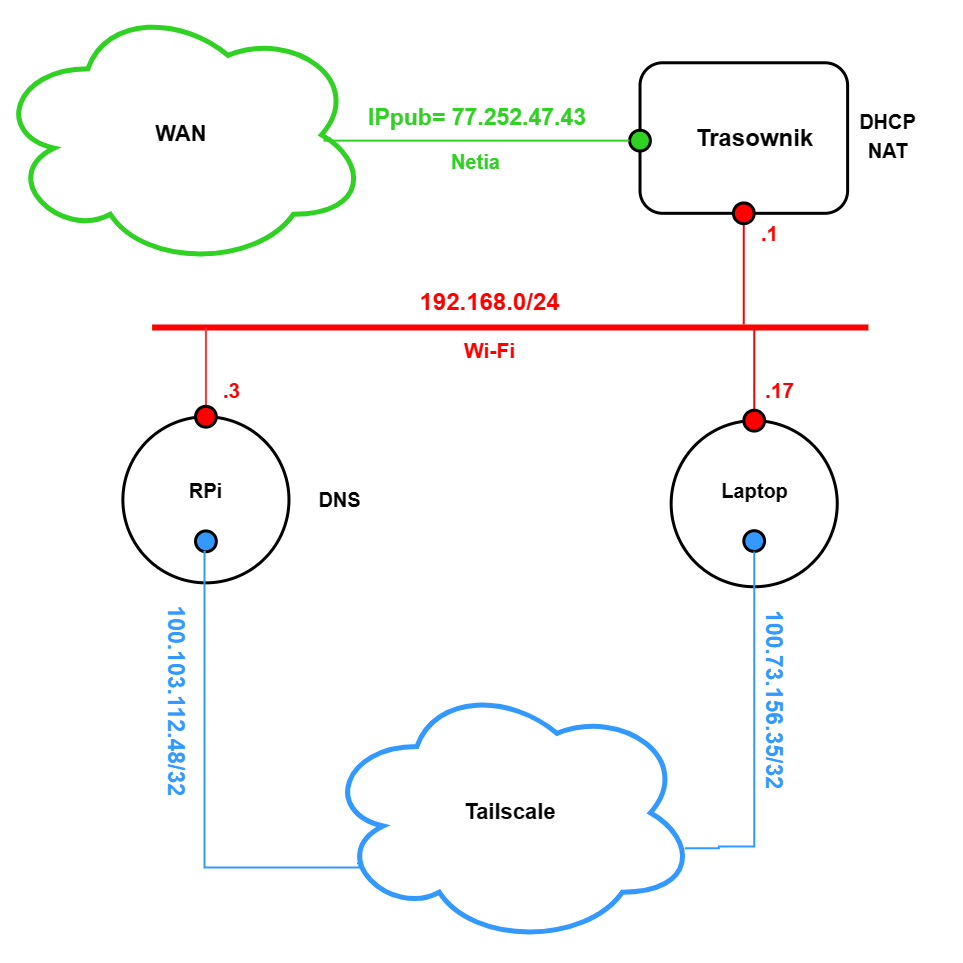
\includegraphics[scale=0.5]{siec3.png}
    \caption{shcemat sieci wykożeystywanej w projekcie}
  \label{fig:siec}
\end{figure}

\section{Analiza sieci}
\subsection*{Raspberry Pi}
\begin{lstlisting}
tkowa@raspberrypi:~ $ ip -c -br l
lo               UNKNOWN        00:00:00:00:00:00 <LOOPBACK,UP,LOWER_UP>
eth0             DOWN           dc:a6:32:2a:26:06 <NO-CARRIER,BROADCAST,MULTICAST,UP>
wlan0            UP             dc:a6:32:2a:26:07 <BROADCAST,MULTICAST,UP,LOWER_UP>
tailscale0       UNKNOWN        <POINTOPOINT,MULTICAST,NOARP,UP,LOWER_UP>

tkowa@raspberrypi:~ $ ip -c -br -4 a
lo               UNKNOWN        127.0.0.1/8
wlan0            UP             192.168.0.3/24
tailscale0       UNKNOWN        100.103.112.48/32

tkowa@raspberrypi:~ $ ip -c -br -6 a
lo               UNKNOWN        ::1/128
wlan0            UP             fe80::312e:69b8:2c16:d4ed/64
tailscale0       UNKNOWN        fd7a:115c:a1e0:ab12:4843:cd96:6267:7030/128
fe80::6bdb:fc4f:49bf:9d27/64
\end{lstlisting}
Warto w tym miejscu zauważyć że maska na interfejsie tailscale0 dla IPv4 wynosi 32. Oznacza to adres jest indywidualny i nie należy do żadnej sieci. Trzeba pamiętać że tailscale jest oprgramowaniem które ma zapisane na serwerach jak które użądzenie jest w jakiej sieci, dlatego nie ma problemu z łączeniem się z nimi.

Kolejnym spostrzeniem jest, że adres IPv6 interfejsu wlan0 znajduje się w podsieci wraz z adresem interfejsu tailscale0. W tej podsieci może ystępować dialog między owymi interfejsami. 

\begin{lstlisting}
tkowa@raspberrypi:~ $ ip -c -br -4 r
default via 192.168.0.1 dev wlan0 src 192.168.0.3 metric 303
192.168.0.0/24 dev wlan0 proto dhcp scope link src 192.168.0.3 metric 303

tkowa@raspberrypi:~ $ ip -c -br -6 r
::1 dev lo proto kernel metric 256 pref medium
fd7a:115c:a1e0:ab12:4843:cd96:6267:7030 dev tailscale0 proto kernel metric 256 pref medium
fe80::/64 dev tailscale0 proto kernel metric 256 pref medium
fe80::/64 dev wlan0 proto kernel metric 256 pref medium
\end{lstlisting}

W sieci dostępne są dwie trasy dla IPv4 oraz cztery trasy dla IPv6:
\begin{enumerate}[label=\textbullet]
  \item jedna z nich jest domyślna (default) skierowana do 192.168.0.1 przez interfejs wlan0. Źródłowy adres IP dla tej trasy to 192.168.0.3, a metryka wynosi 303
  \item druga jest dla lokalnej podsieci 192.168.0.0/24, która jest dostępna przez interfejs wlan0. Źródłowy adres IP dla tej trasy to 192.168.0.3, a metryka wynosi 303
  \item ::1 dev lo proto kernel metric 256 pref medium - Ta trasa jest dla lokalnego interfejsu pętli zwrotnej (loopback) o adresie ::1. Ma metrykę 256 i priorytet medium.
  \item fd7a:115c:a1e0:ab12:4843:cd96:6267:7030 dev tailscale0 proto kernel metric 256 pref medium - Ta trasa jest dla interfejsu tailscale0 o adresie fd7a:115c:a1e0:ab12:4843:cd96:6267:7030. Ma metrykę 256 i priorytet medium.
  \item fe80::/64 dev tailscale0 proto kernel metric 256 pref medium - Ta trasa jest dla interfejsu tailscale0 dla podsieci fe80::/64. Ma metrykę 256 i priorytet medium.
  \item fe80::/64 dev wlan0 proto kernel metric 256 pref medium - Ta trasa jest dla interfejsu wlan0 dla podsieci fe80::/64. Ma metrykę 256 i priorytet medium.
\end{enumerate}
Trasa dla lokalnej podsieci 192.168.0.0/24 jest używana dla komunikacji wewnątrz niej bez bramy, natomiast domyślna trasa (default) służy do przekazywania ruchu, który nie jest skierowany do tej lokalnej podsieci, przez bramę o adresie 192.168.0.1. Obie trasy mają taką samą metrykę (303), co oznacza, że mają taki sam priorytet i ruch może być przekazywany zarówno przez trasę lokalnej podsieci, jak i przez domyślną trasę, w zależności od celu komunikacji.\\

Trasa pętli zwrotnej jest wykorzystywana do przekierowania ruchu sieciowego skierowanego na adres loopback do interfejsu pętli zwrotnej w celu lokalnego przetwarzania. Kolejna trasa wskazuje, że ruch skierowany do określonego adresu zostanie przekierowany przez interfejs "tailscale0"do celu zdefiniowanego przez ten adres. Trzecia trasa dla IPv6 odnosi się do lokalnej podsieci fe80::/64, która obejmuje adresy link-local, i jest powiązana z interfejsem "tailscale0". Adresy link-local są używane do komunikacji w obrębie tej samej sieci lokalnej. Wynika z tego, że ruch kierowany do podsieci fe80::/64 zostanie przekierowany przez interfejs "tailscale0". Podobnie, trasa sieciowa fe80::/64, również należąca do lokalnej podsieci fe80::/64, jest skojarzona z interfejsem "wlan0", który zazwyczaj służy do bezprzewodowych połączeń sieciowych. Ta trasa wskazuje, że ruch kierowany do podsieci fe80::/64 będzie przekierowany przez interfejs "wlan0".\\

Zatem komunikacja między interfejsam wlan0 oraz Tailscale odbywa się w podsieci fe80::/64. Jeśli łączymy się przez tailscale to tamtędy przebiega trasa łączenia się z Raspberry.\cite{stevens1994tcp}

\subsection*{Laptop}
\begin{lstlisting}
PS C:\Users\tkowa> Get-NetIPAddress -AddressFamily IPv4
...
IPAddress         : 192.168.0.17
InterfaceAlias    : Wi-Fi
PrefixLength      : 24

IPAddress         : 100.73.156.35
InterfaceAlias    : Tailscale
PrefixLength      : 32
...

PS C:\Users\tkowa> Get-NetIPAddress -AddressFamily IPv6
...
IPAddress         : fe80::2979:57de:62a:5bd7
InterfaceAlias    : Wi-Fi
PrefixLength      : 64

IPAddress         : fe80::d8ff:5060:f230:9168
InterfaceAlias    : Tailscale
PrefixLength      : 64

IPAddress         : fd7a:115c:a1e0:ab12:4843:cd96:6249:9c23
InterfaceAlias    : Tailscale
PrefixLength      : 128
...
\end{lstlisting}
Interfejs Wi-Fi ma przypisane zarówno adresy IP w wersji IPv4, jak i IPv6. Adres IPv4 to 192.168.0.17 ma maskę 24. Ten adres został przydzielony za pomocą protokołu DHCP. Adres IPv6 to fe80::2979:57de:62a:5bd7 z maską 64 służy do komunikowania się w sieci lokalnej.\\

Interfejs Tailscale również ma adresy IP w wersji IPv4, jak i IPv6. Adres IPv4 to 100.73.156.35 z maską 32 został skonfigurowany ręcznie i służy do komunikowania się w sieci Tailscale. Adres IPv6 to fd7a:115c:a1e0:ab12:4843:cd96:6249:9c23 z maską 128 również został skonfigurowany ręcznie i tak samo używany. Trzeci adres fe80::d8ff:5060:f230:9168 tak jak w przypadku Wi-Fi służy do komunikacj w sieci lokalnej.

\begin{lstlisting}
PS C:\Users\tkowa> Get-NetRoute | Where-Object {$_.InterfaceAlias -eq 'Wi-Fi'}

ifInd DestinationPrefix                           NextHop  RouteMetric Metric PolicyStore
----- -----------------                           -------  ----------- ------ -----------
9     255.255.255.255/32                          0.0.0.0          256 55     ActiveStore
9     224.0.0.0/4                                 0.0.0.0          256 55     ActiveStore
9     192.168.0.255/32                            0.0.0.0          256 55     ActiveStore
9     192.168.0.17/32                             0.0.0.0          256 55     ActiveStore
9     192.168.0.0/24                              0.0.0.0          256 55     ActiveStore
9     0.0.0.0/0                                   192.168.0.1        0 55     ActiveStore
9     ff00::/8                                    ::               256 55     ActiveStore
9     fe80::2979:57de:62a:5bd7/128                ::               256 55     ActiveStore
9     fe80::/64                                   ::               256 55     ActiveStore

\end{lstlisting}
\clearpage
\begin{lstlisting}
  PS C:\Users\tkowa> Get-NetRoute | Where-Object {$_.InterfaceAlias -eq 'Tailscale'}

ifInd DestinationPrefix                           NextHop  RouteMetric Metric PolicyStore
----- -----------------                           -------  ----------- ------ -----------
51    100.103.112.48/32                           0.0.0.0            0 5      ActiveStore
51    100.100.100.100/32                          0.0.0.0            0 5      ActiveStore
51    100.75.222.28/32                            0.0.0.0            0 5      ActiveStore
51    100.73.156.35/32                            0.0.0.0          256 5      ActiveStore
51    fd7a:115c:a1e0:ab12:4843:cd96:6249:9c23/128 ::               256 5      ActiveStore
51    fd7a:115c:a1e0::/48                         ::                 0 5      ActiveStore
  
\end{lstlisting}


Dla interfejsu Wi-Fi istnieje wpis dla domyślnej trasy (0.0.0.0/0), który wskazuje na bramę sieciową o adresie 192.168.0.1. Tablica tras również zawiera wpisy dla ruchu lokalnego w sieci Wi-Fi, takie jak 192.168.0.0/24, 192.168.0.17/32, które określają zasięg sieci i trasowanie ruchu w obrębie tej sieci.\\

Dla interfejsu Tailscale również istnieje tablica tras zawierająca wpisy dotyczące ruchu w tej sieci. Wpis dla ruchu do adresu 100.73.156.35/32 wskazuje, że ruch lokalny jest kierowany bezpośrednio do tego adresu. Ponadto, istnieją wpisy dotyczące ruchu w sieci IPv6, takie jak fd7a:115c:a1e0:ab12:4843:cd96:6249:9c23/128, fd7a:115c:a1e0::/48, które określają trasowanie ruchu w sieci IPv6 w ramach Tailscale.\\

\section{Wydajność}
\subsection*{NAS1}
Dysk sieciowy został skutecznie zmapowany na moim laptopie, umożliwiając łatwy dostęp do jego zawartości. Dodatkowo, używając IP Tailscale, zmapowałem ten sam dysk, co umożliwia dostęp do niego jedynie poprzez połączenie internetowe.\\

Postanowiłem przetestować efektywność przesyłania plików z mojego laptopa na dysk oraz czas pobierania plików z tego dysku, korzystając z poleceń PowerShell. Przeprowadziłem te testy dla interfejsów wlan0 oraz Tailscale, a oto wyniki, które uzyskałem:\\

\begin {table} [H]
    \begin {center}

        \label {Tabela 3}
        \begin {tabular} { |c|r|r| }
            \hline
            Przybliżona waga pliku & przesyłanie & pobieranie \\
            \hline
            700MB & 256,125s & 189,028s \\
            \hline
            50MB & 12,559s & 10,606s \\
            \hline
            1MB & 3,167s & 0,585s \\
            \hline
            0.01MB & 0,289s & 0,091s \\
            \hline
        \end {tabular}
        \caption {interfejs wlan0}
    \end {center}
\end {table}

\begin {table} [H]
    \begin {center}

        \label {Tabela 3}
        \begin {tabular} { |c|r|r| }
            \hline
            Przybliżona waga pliku & przesyłanie & pobieranie \\
            \hline
            700MB & 312,232s & 193,062s \\
            \hline
            50MB & 15,614s & 11,500s \\
            \hline
            1MB & 4,336s & 0,809s \\
            \hline
            0.01MB & 0,323s & 0,234s \\
            \hline
        \end {tabular}
        \caption {interfejs Tailscale}
    \end {center}
\end {table}
Dzięki temu porównaniu można dokładniej ocenić wydajność obu interfejsów podczas przesyłania i pobierania plików. Wyraźnie widać, że dla Tailscale’a wyniki są nieco gorsze, czego przyczyną jest korzystanie z sieci wewnętrznej i różnych punktów dostępowych.\\

Średni czas przesyłania plików na dysk wynosi około 3,3 MB/s dla interfejsu wlan0 i 2,1 MB/s dla Tailscale. Pomimo tych nieco niższych prędkości, dla zastosowań domowych, takich jak przesyłanie zdjęć z wyjazdu czy krótkich filmów, jest to wystarczające.\\

Uśredniony czas pobierania plików jest szybszy niż czas przesyłania i wynosi około 4,2 MB/s dla interfejsu wlan0 oraz 3,9 MB/s dla Tailscale. Dzięki temu, można swobodnie przechowywać filmy na dysku i poczekać chwilę, aż się pobiorą, aby można było je obejrzeć w dowolnym miejscu.\\

Warto zauważyć, że lepiej jest pobierać film na jakiś czas niż oglądać go bezpośrednio z dysku, ponieważ mogą wystąpić problemy z siecią, powodujące zacinanie się filmu. Natomiast po pobraniu filmu, można go szybko odtworzyć, niezależnie od stabilności sieci.\\

Należy również pamiętać, że obecnie funkcję przechowywania plików pełni pendrive, który nie zapewnia takiej wydajności jak dysk SSD lub HDD. Warto rozważyć zastosowanie szybszego dysku, który zwiększy prędkość transferu danych oraz zapewni większą pojemność przechowywania plików.

\subsection*{Blokada reklam}
Do testowania wydajności Pi-hole skorzystałem z łatwo dostępnej strony internetowej \href{https://d3ward.github.io/toolz/adblock.html}{d3ward}. Jest to prosty w obsłudze serwis, który po wejściu na stronę od razu rozpoczyna testowanie. Możliwość powtórzenia testu po zakończeniu pozwala na lepszą analizę wyników. Jeśli chcemy przyjrzeć się bardziej szczegółowo, jakie elementy nie zostały zablokowane, oraz znaleźć listy, które mogłyby je uzupełnić, mamy pełen dostęp do wyników.\\

Przeprowadzam testowanie w dwóch wariantach. Pierwszy obejmuje użycie wszystkich dodanych list blokujących. Dzięki temu możemy sprawdzić, jak skutecznie system radzi sobie z blokowaniem różnych typów treści. Drugi wariant polega na odblokowaniu tych list, co pozwala nam zobaczyć, jakie elementy mogą przejść przez system, można nazwać to próbą kontrolną, tak jab by Pi-hole nie działało.\cite{piholeBLog}

\begin{figure}[H]
  \centering
  \begin{minipage}{0.5\textwidth}
    \centering
    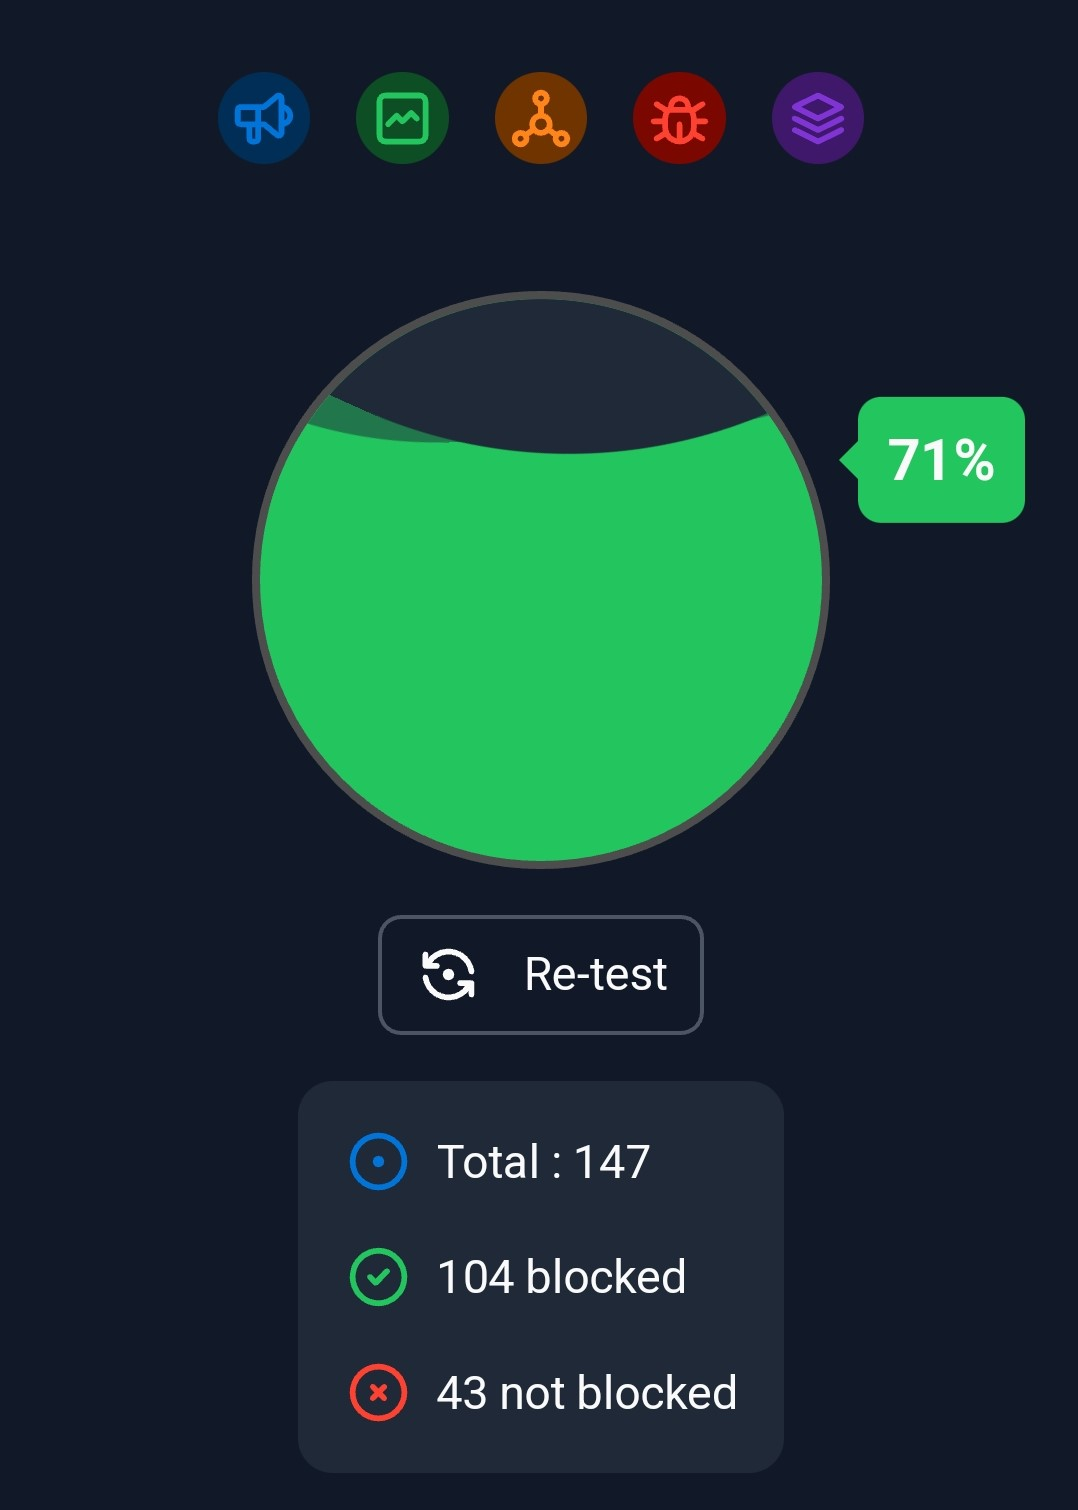
\includegraphics[scale=0.2]{zBlokem1.jpg}
    \caption{z zablokowanymi domenami}
  \end{minipage}\hfill
  \begin{minipage}{0.5\textwidth}
    \centering
    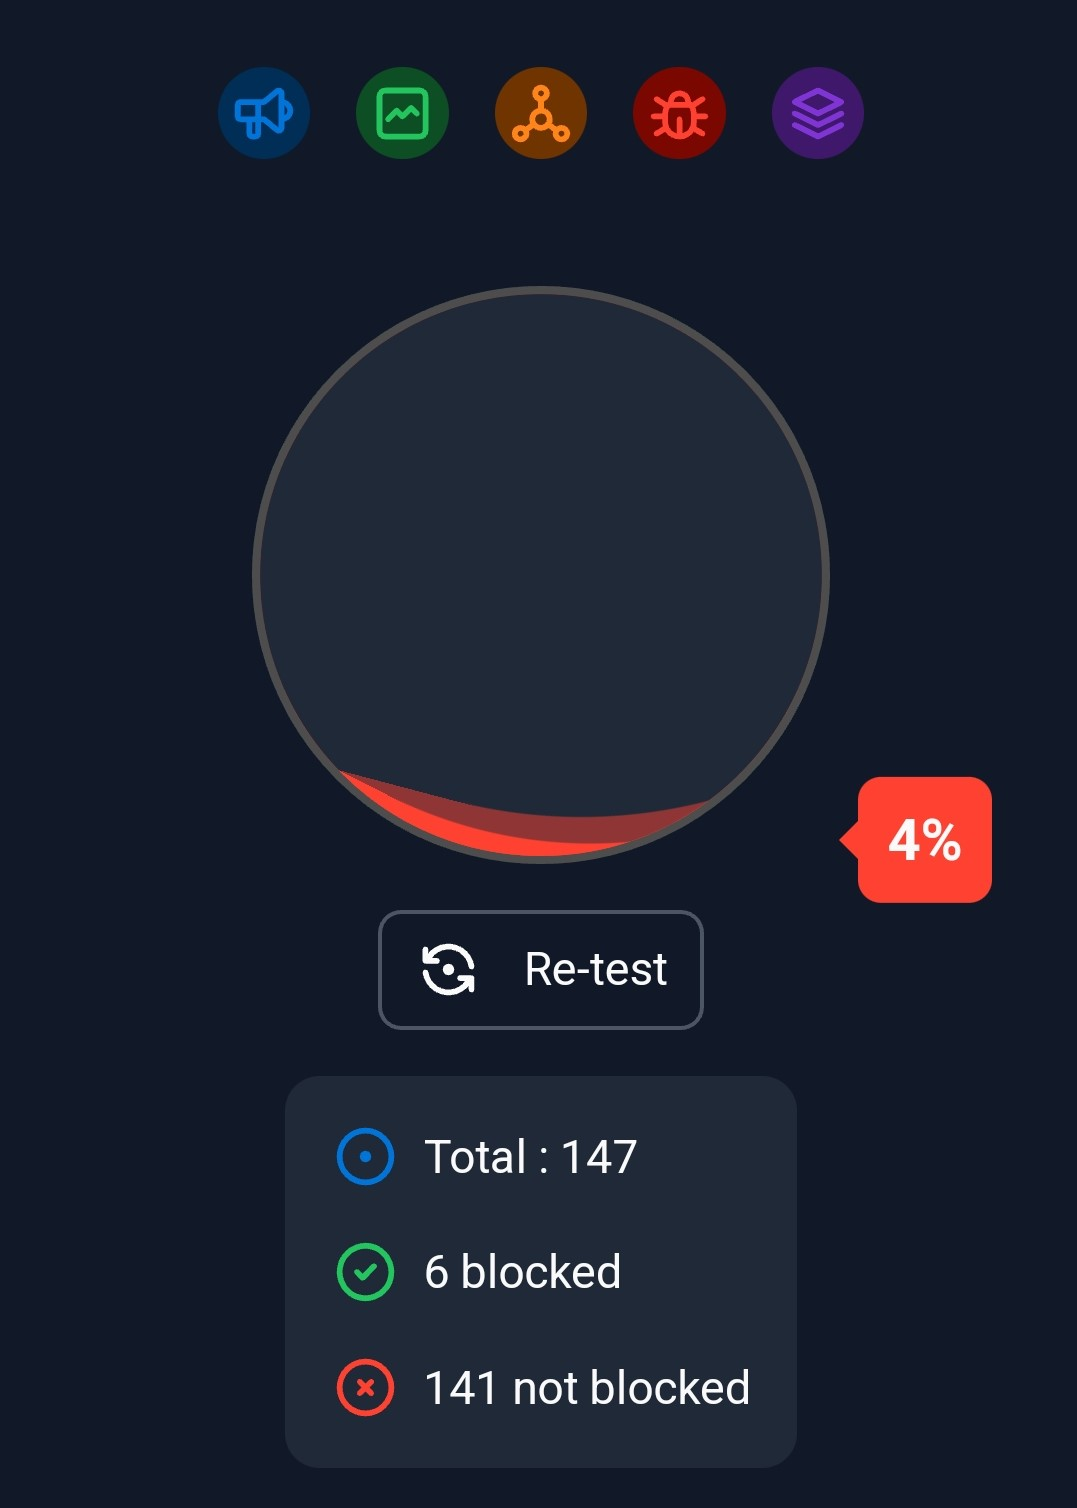
\includegraphics[scale=0.2]{bezBloka1.jpg}
    \caption{bez blokowania domen}
  \end{minipage}
\end{figure}

Wyniki testów wyraźnie pokazują, że Pi-hole dobrze spełnia swoją funkcję. Zastosowanie Pi-hole powodowało zablokowanie aż 71\% niechcianych elementów, podczas gdy bez Pi-hole tylko 4\% zostało zablokowanych. Wyniki pokazują, że narzędzie ma duży procent skuteczności przy blokowaniu podejrzanych witryn.\\

Warto zauważyć, że Pi-hole może zwiększyć swoja skuteczność poprzez dodanie kolejnych list blokujących. Jednak w obecnej konfiguracji jego wydajność jest zdecydowanie wystarczająca. Jest to szczególnie widoczne podczas korzystania z telefonu w sieci domowej lub poza nią, gdzie mnóstwo reklam pojawia się na stronach internetowych.\\

Jednak każda kolejna lista blokująca skutkuje większą liczbą zablokowanych stron. Dlatego ważne jest zachowanie ostrożności, aby nie zablokować zbyt dużej części Internetu, co zakłóca swobodne korzystanie z urządzeń. Staranne wybieranie list blokujących zapewnia zarówno skuteczną ochronę przed reklamami i swobodny dostępu do pożądanych treści.
\section{Wnioski}

W moim przypadku, dysk sieciowy, który utworzyłem, jest głównie wykorzystywany do transferu plików między laptopem a Raspberry Pi. Na razie korzystam z pendrive’a o pojemności 16 GB, ale niedługo planuję zastąpić go dyskiem SSD o pojemności 1 TB. Chcę, żeby nowy dysk zawierał zdjęcia i dokumenty rodzinne oraz był dostępny dla pozostałych domowników. Dlatego będę dodawać kolejne urządzenia do mojej sieci Tailscale, żeby umożliwić im swobodny dostęp do tego dysku.\\

Moja sieć domowa jest teraz lepiej zabezpieczona dzięki Pi-hole, oprogramowaniu, które jest warte polecenia. Poza pracą z linii poleceń mogłem skorzystać z czytelnego interfejsu graficznego, który ułatwia nawigację i konfigurację. Pi-hole posiada również rozbudowaną dokumentację, która była dla pomocna w mojej pracy. Dzięki niej łatwo mogłem znaleźć informacje i przykłady dotyczące różnych funkcji. Kiedy moje pytania dotyczyły informacji z poza dokumentacji, mogłem zadać je pomocy Pi-hole, gdzie znalazłem wiele odpowiedzi.\\

Praca nad tym projektem wiele mi dała. Nauczyłem się korzystania z linii poleceń, pisania podstawowych skryptów w języku shell oraz lepiej zrozumiałem system Linux. Będę mógł wykorzystać te umiejętności w moich kolejnych projektach. Dodatkowo nauczyłem się pisać prace w LaTeX, co pozwoli mi tworzyć profesjonalne sprawozdania i dokumenty w przyszłości. Projekt poprawił bezpieczeństwo mojej sieci domowej i sposobu przechowywania danych, również poszerzył moje umiejętności techniczne i wiedzę z tego obszaru informatyki.

\bibliographystyle{IEEEtran}
\bibliography{bibl}
\clearpage
\section*{Skrypty}
Wszyskie skrypty muza być wykonywane z uprawnieniami administratora. Wystarczy wpisać:\\
\textit{sudo ./nazwa\_skryptu.sh}\cite{ytScript}

\begin{lstlisting}[caption={skrypt konfiguracyjny Paspberry Pi: \textit{basic\_config.sh}}]

#!/bin/sh
#podstawowa konfiguracja RPi4
#tkowa 05.2023

# Zmienne konfiguracyjne
interface="wlan0"
static_ip_address="192.168.0.3/24"
static_routers="192.168.0.1"
static_domain_name_servers="192.168.0.3 8.8.8.8"
ssid="StudPW-ubnRvpT-2.4G"
psk="hasloDoSieci"

cp /etc/dhcpcd.conf /etc/dhcpcd.conf.old

echo '' >> /etc/dhcpcd.conf
echo "# Konfiguracja statyczna dla interfejsu $interface" >> /etc/dhcpcd.conf
echo "interface $interface" >> /etc/dhcpcd.conf
echo "static ip_address=$static_ip_address" >> /etc/dhcpcd.conf
echo "static routers=$static_routers" >> /etc/dhcpcd.conf
echo "static domain_name_servers=$static_domain_name_servers" >> /etc/dhcpcd.conf

echo '' >> /etc/wpa_supplicant/wpa_supplicant.conf
echo "# Sieć $ssid" >> /etc/wpa_supplicant/wpa_supplicant.conf
echo "network={" >> /etc/wpa_supplicant/wpa_supplicant.conf
echo "    ssid=\"$ssid\"" >> /etc/wpa_supplicant/wpa_supplicant.conf
echo "    psk=\"$psk\"" >> /etc/wpa_supplicant/wpa_supplicant.conf
echo "}" >> /etc/wpa_supplicant/wpa_supplicant.conf

rfkill unblock 0
ifconfig $interface up

systemctl enable ssh
systemctl start ssh

reboot
\end{lstlisting}
\clearpage

\begin{lstlisting}[caption={skrypt konfiguracyjny NAS: \textit{nas1\_config.sh}}]
#!/bin/sh
#utwożenie dysku NAS
#tkowa 05.2023

if [ -z "$1" ] || [ -z "$2" ]; then
  echo "Podaj nazwe uzytkownika i sciezke dysku jako argumenty."
  exit 1
fi

username=$1
disc_location=$2

if [ ! -d "$disc_location" ]; then
  echo "Podana scieżka dysku ($disc_location) jest niedostępna."
  exit 1
fi

uid=$(id -u "$username")
if [ $? -eq 0 ]; then
else
  echo "Nie mozna odnalezc uzytkownika: $username"
  exit 1
fi

gid=$(id -g "$username")
if [ $? -eq 0 ]; then
else
  echo "Nie można odnaleźć grupy użytkownika dla: $username"
  exit 1
fi

mkdir /media/NAS1
cp /etc/fstab /etc/fstab.old
echo "$2        /media/NAS1     auto uid=$uid,gid=$gid,noatime 0 0" >> /etc/fstab
echo "" >> /etc/fstab
mount -a

cp /etc/samba/smb.conf /etc/samba/smb.conf.old
echo "" >> /etc/samba/smb.conf
echo "[NAS1]" >> /etc/samba/smb.conf
echo "" >> /etc/samba/smb.conf
echo "  path = /media/NAS1" >> /etc/samba/smb.conf
echo "  valid users = @users" >> /etc/samba/smb.conf
echo "  force group = users" >> /etc/samba/smb.conf
echo "  create mask = 0660" >> /etc/samba/smb.conf
echo "  directory mask = 0771" >> /etc/samba/smb.conf
echo "  read only = on" >> /etc/samba/smb.conf
echo "  guest ok = on" >> /etc/samba/smb.conf
echo "  writeable = on" >> /etc/samba/smb.conf

service smbd restart
\end{lstlisting}
\clearpage

\begin{lstlisting}[caption={skrypt konfiguracyjny Pi-hole: \textit{pihole\_config.sh}}]
#!/bin/sh

nazwa_pliku="pewien_napis"
napis_do_usuniecia="tekst_do_usuniecia"

while [ $# -gt 0 ]; do
  key="$1"

  case $key in
    -h)
      # Help
      echo "-k                  konfiguracja"
      echo "-add [link] *[kom]   dodanie listy blokującej"
      echo "-h                  pomoc"
      echo "* komentarz nie jest obowiazkowy"
      ;;
    -k)
      touch /etc/unbound/unbound.conf.d/pi-hole.conf
      cat <<EOF > "/etc/unbound/unbound.conf.d/pi-hole.conf"
server:
    # If no logfile is specified, syslog is used
    # logfile: "/var/log/unbound/unbound.log"
    verbosity: 0

    interface: 127.0.0.1
    port: 5335
    do-ip4: yes
    do-udp: yes
    do-tcp: yes

    # May be set to yes if you have IPv6 connectivity
    do-ip6: no

    # You want to leave this to no unless you have *native* IPv6. With 6to4 and
    # Terredo tunnels your web browser should favor IPv4 for the same reasons
    prefer-ip6: no

    # Use this only when you downloaded the list of primary root servers!
    # If you use the default dns-root-data package, unbound will find it automatically
    #root-hints: "/var/lib/unbound/root.hints"

    # Trust glue only if it is within the server's authority
    harden-glue: yes

    # Require DNSSEC data for trust-anchored zones, if such data is absent, the zone becomes BOGUS
    harden-dnssec-stripped: yes

    # Don't use Capitalization randomization as it known to cause DNSSEC issues sometimes
    # see https://discourse.pi-hole.net/t/unbound-stubby-or-dnscrypt-proxy/9378 for further details
    use-caps-for-id: no

    # Reduce EDNS reassembly buffer size.
    # IP fragmentation is unreliable on the Internet today, and can cause
    # transmission failures when large DNS messages are sent via UDP. Even
    # when fragmentation does work, it may not be secure; it is theoretically
    # possible to spoof parts of a fragmented DNS message, without easy
    # detection at the receiving end. Recently, there was an excellent study
    # >>> Defragmenting DNS - Determining the optimal maximum UDP response size for DNS <<<
    # by Axel Koolhaas, and Tjeerd Slokker (https://indico.dns-oarc.net/event/36/contributions/776/)
    # in collaboration with NLnet Labs explored DNS using real world data from the
    # the RIPE Atlas probes and the researchers suggested different values for
    # IPv4 and IPv6 and in different scenarios. They advise that servers should
    # be configured to limit DNS messages sent over UDP to a size that will not
    # trigger fragmentation on typical network links. DNS servers can switch
    # from UDP to TCP when a DNS response is too big to fit in this limited
    # buffer size. This value has also been suggested in DNS Flag Day 2020.
    edns-buffer-size: 1232

    # Perform prefetching of close to expired message cache entries
    # This only applies to domains that have been frequently queried
    prefetch: yes

    # One thread should be sufficient, can be increased on beefy machines. In reality for most users running on small networks or on a single machine, it should be unnecessary to seek performance enhancement by increasing num-threads above 1.
    num-threads: 1

    # Ensure kernel buffer is large enough to not lose messages in traffic spikes
    so-rcvbuf: 1m

    # Ensure privacy of local IP ranges
    private-address: 192.168.0.0/16
    private-address: 169.254.0.0/16
    private-address: 172.16.0.0/12
    private-address: 10.0.0.0/8
    private-address: fd00::/8
    private-address: fe80::/10
EOF
      sed -i '/PIHOLE_DNS/d' "/etc/pihole/setupVars.conf"
      echo "PIHOLE_DNS_1=127.0.0.1#5335" >> /etc/pihole/setupVars.conf
      service unbound restart
      ;;
    -add)
      if [ -n "$2" ]; then
        lista_blokujaca="$2"
        echo "Dodaje link: $lista_blokujaca"
        if [ -n "$3" ]; then
          komentarz="$3"
          sqlite3 /etc/pihole/gravity.db "INSERT INTO adlist (address, enabled, comment)
          VALUES ('$lista_blokujaca', 1, '$komentarz');"
        else
          sqlite3 /etc/pihole/gravity.db "INSERT INTO adlist (address, enabled, comment)
          VALUES ('$lista_blokujaca', 1, 'NOWA');"
        fi
        shift 2
      else
        echo "Blad: Drugi argument nie zostal dostarczony."
        return 1
      fi
      ;;
    *)
      echo "Nieznana opcja: $key"
      ;;
  esac
  shift
done
\end{lstlisting}
\end{document}
